%----------------------------------------------------------------------------------------------------------------------------------------------------------%
\chapter{Physical experimentation}
%----------------------------------------------------------------------------------------------------------------------------------------------------------%
\section{Description}
\paragraph{}This experiment looks at finding out the prevalence of \emph{Staphylococcus Aureus} in a sample of students from the school. The process used involves extracting a sample from underneath a subject's nalis by swabbing, cultivating that sample and then observing the results of said culture to determine the presence or not of Staphylococcus Aureus as part of the subject's resident bacterial flora. Each iteration of the process took less than two minutes to complete. However, all the safety measures and actions taken need more time to be taken care of properly. 
%----------------------------------------------------------------------------------------------------------------------------------------------------------%
\section{Protocol followed}
\paragraph{}The protocol followed was designed based on a similar protocol used in the many university laboratories\cite{olearyPracticalHandbookMicrobiology1989}, modified to fit the needs of this research paper, and peer-reviewed by Olga Sánchez, and uploaded to the Protocols.io platform, to make it easier to follow the days of that the experiment took place in. This protocol underwent 9 different revisions\cite{rocacugatStaphilococcusAureusSampling2022a}. It can also be read below:
\begin{enumerate}
\item
\end{enumerate}•
%----------------------------------------------------------------------------------------------------------------------------------------------------------%
\section{Bill of materials}
\paragraph{}The materials used, as well as the quantities used can be found in the following table. On the left, laboratory equipment and, on the right, regents and consumables used:
\begin{figure}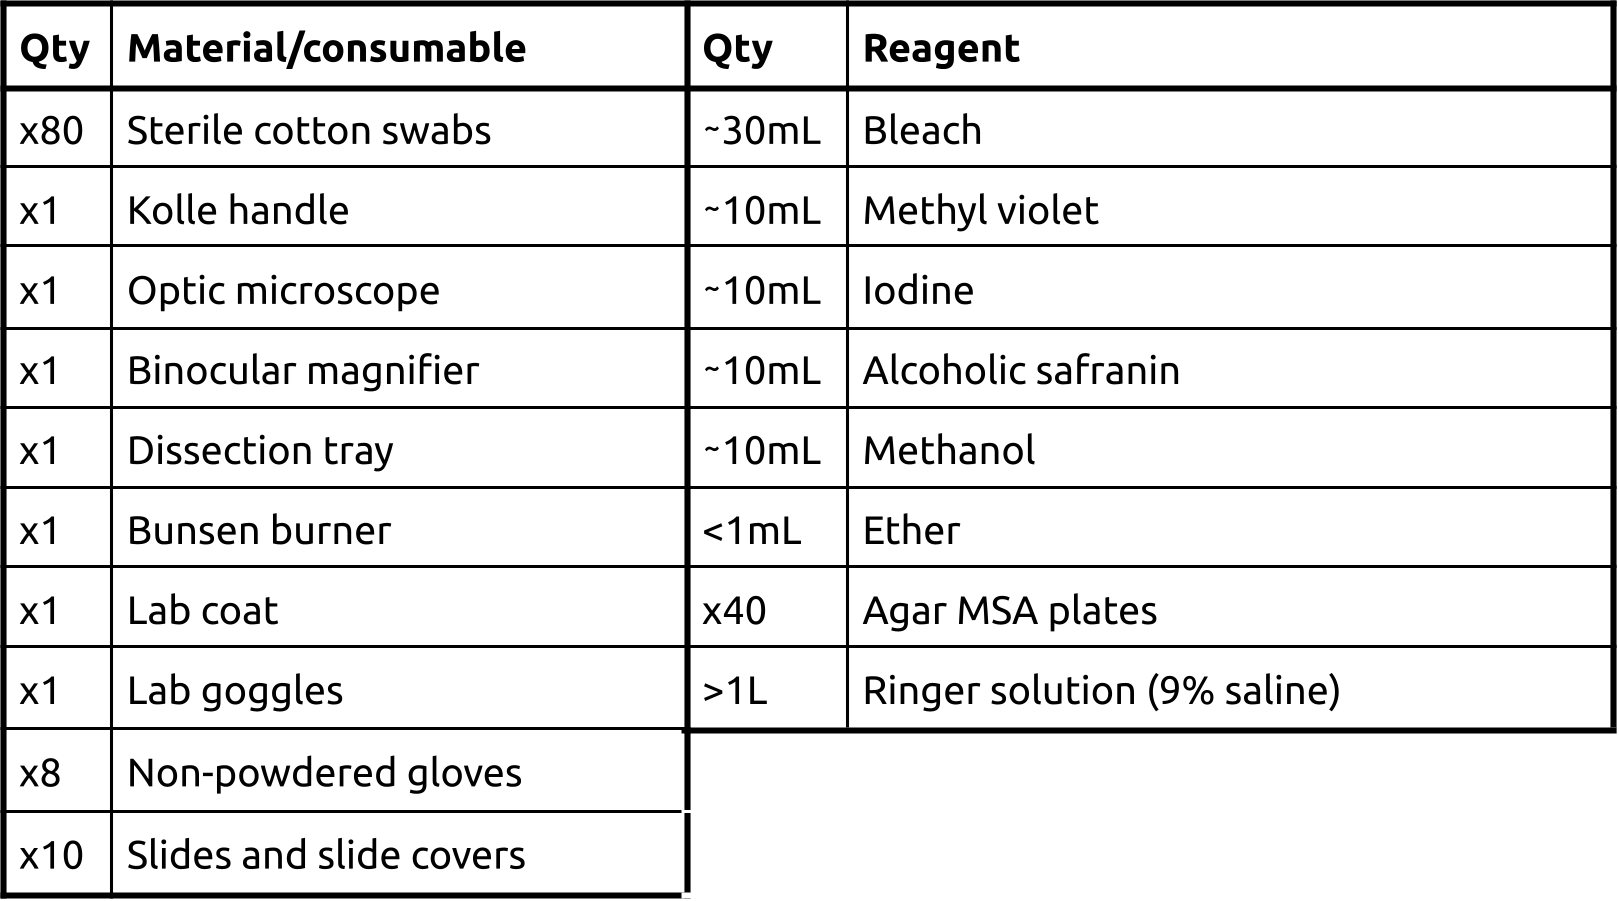
\includegraphics[width=0.48\textwidth]{BOM-1.png}\end{figure}
%----------------------------------------------------------------------------------------------------------------------------------------------------------%
\section{Risk assessment and prevention}
\paragraph{}Staph is considered a Biosecurity Level (BSL) 2 pathogenic bacteria. This means that the it is associated with a human disease that can pose a moderate human health hazard. In a laboratory where BSL-2 pathogens are handled, regular lab rules should be followed (mechanical pipetting only, hand washing, prohibiting the consumption of food and drinks in the lab, proper PPE use...), as well as avoiding splashes or aerosols, biohazard warning signs present on all material used, as well as proper surface and material disinfection via the use of autoclave or alternative decontamination method.[source: book] The risks associated with this bacteria were assessed following the protocol designated by the World Health Organisation [cite], and proper security measures were followed at all times when handling biohazardous material. No incidents occurred during the research part of this project, and the protocol defined previous to the start was followed to a T. While the laboratory used may not be the most ideal type of laboratory for this type of research, it is certainly adequate enough to perform a research project like this one